\RequirePackage{fix-cm}
\documentclass[smallextended]{svjour3}       % onecolumn (second format)
\smartqed  % flush right qed marks, e.g. at end of proof
\usepackage{graphicx}
%
% \usepackage{mathptmx}      % use Times fonts if available on your TeX system
%
% insert here the call for the packages your document requires
%\usepackage{latexsym}
\usepackage{tikz}     % For adding axes to plots
\usetikzlibrary{positioning}
\usepackage{graphicx} % For including PDFs
\usepackage{amsmath} % assumes amsmath package installed
\usepackage{amssymb}  % assumes amsmath package installed
\usepackage{booktabs} % For formal tables

%
% please place your own definitions here and don't use \def but
% \newcommand{}{}

%% Command for creating multiplie-line cells inside a table environment
\newcommand{\multilinecell}[2][c]{%
  \begin{tabular}[#1]{@{}c@{}}#2\end{tabular}}

%% \newcommand{\Bigl}{\mathopen\Big}
%% \newcommand{\Bigr}{\mathclose\Big}
%
% Insert the name of "your journal" with
\journalname{Numerical Algorithms}
%
\begin{document}

\title{Interpolation of Sparse High-Dimensional Data\thanks{This
    projected was supported by NSF grant}
}
% \subtitle{Do you have a subtitle?\\ If so, write it here}

%\titlerunning{Short form of title}        % if too long for running head

\author{Thomas C. H. Lux   \and
  Layne T. Watson          \and
  Tyler H. Chang           \and
  Yili Hong                \and
  Kirk Cameron
}

%\authorrunning{Short form of author list} % if too long for running head

\institute{Thomas Lux \at
  Virginia Polytechnic Institute \& State University (VPI\&SU) \\
  Blacksburg, VA 24061 \\
  \email{tchlux@vt.edu}
}

\date{Received: date / Accepted: date}
% The correct dates will be entered by the editor

\maketitle

\begin{abstract}
A rapid increase in the quantity of data available is allowing all fields of science to generate more accurate models of multivariate phenomena. Regression and interpolation become challenging when the dimension of data is large, especially while maintaining tractable computational complexity. While regression is a popular approach to solving approximation problems with high dimension, there are often advantages to interpolation. This paper presents error bounds for interpolants on moderately high dimensional problems and contrasts their performance with that of popular regression techniques. Empirical results demonstrate the viability of interpolants for high dimensional approximation problems, suggesting that these techniques are capable of effectively modeling multivariate phenomena while maintaining flexibility in different application domains.

\keywords{approximation \and regression \and interpolation \and high dimension \and error bound}
% \PACS{PACS code1 \and PACS code2 \and more}
% \subclass{MSC code1 \and MSC code2 \and more}
\end{abstract}

%     Introduction     
%======================

\section{Introduction}
\label{sec:introduction}

Regression and interpolation are problems of considerable importance that find applications across many fields of science. Pollution and air quality analysis \cite{de2008field}, energy consumption management \cite{lazos2014optimisation}, and student performance prediction \cite{cortez2008using,lux2016applications} are a few of many interdisciplinary applications of multivariate regression for predictive analysis. As discussed later, these techniques can also be applied to prediction problems related to high performance computing (HPC) file input/output (I/O) \cite{lux2018nonparametric}, Parkinson's patient clinical evaluations \cite{tsanas2010accurate}, and forest fire risk assessment \cite{cortez2007data}.

Regression and interpolation have a considerable theoretical base in one dimension \cite{cheney2009course}. Splines in particular are well understood as an interpolation technique in one dimension \cite{de1978practical}, particularly B-splines. Tensor products of B-splines \cite{unther1996interpolating} or other basis functions have an unfortunate exponential scaling with increasing dimension. Exponential scaling prohibits tensor products from being reasonably applied beyond three-dimensional data. In order to address this dimensional scaling challenge, C. de Boor and others proposed box splines \cite{de2013box}, of which one of the approximation techniques in this work is composed \cite{lux2018novel}.

The theoretical foundation of low dimensional interpolation allows the construction of strong error bounds that are absent from high dimensional problems. This work extends some known results regarding the secant method \cite{dennis1996numerical} to construct an interpolation error bound for problems of arbitrary dimension. These error bounds are useful, considering the same cannot be said for regression algorithms in general. The maximum complexity of an interpolant is bounded by the amount of data available, while the maximum complexity of a regressor is bounded by both the amount of data and the chosen parametric form. For this reason, generic uniform bounds are largely unobtainable for regression techniques on arbitrary approximation problems, even when the approximation domain is bounded.

Aside from theoretical motivation for the use of interpolants, there are often computational advantages as well. Interpolants do not have the need for \textit{fitting} data, or minimizing error with respect to model parameters. In applications where the amount of data is large and the relative number of predictions that need to be made for a given collection of data is small, the direct application of an interpolant is much less computationally expensive.

In this work, multivariate interpolation is defined given a closed convex subset $Y$ of a metrizable topological vector space with metric $s$, some function $f:\mathbb{R}^d \rightarrow Y$ and a set of points $X = \bigl\{x^{(1)}$,$\ldots$,$x^{(n)}\bigr\} \subset \mathbb{R}^d,$ along with associated function values $f\bigl(x^{(i)}\bigr)$. The goal is to construct an approximation $\hat f: \mathbb{R}^d \rightarrow Y$ such that $\hat f\bigl(x^{(i)}\bigr) = f\bigl(x^{(i)}\bigr)$ for all $i = 1$,$\ldots$,$n$. It is often the case that the form of the true underlying function $f$ is unknown, however it is still desirable to construct an approximation $\hat f$ with small approximation error at $y \notin X$. The two metric spaces that will be discussed in this work are the real numbers with metric $s(x,y) = |x-y|$, and the set of cumulative distribution functions (CDFs) with the Kolmogorov-Smirnov (KS) statistic as metric.

Multivariate regression is often used when the underlying function is presumed to be stochastic, or stochastic error is introduced in the evaluation of $f$. Hence, multivariate regression relaxes the conditions of interpolation by choosing parameters $P$ defining $\hat f(x;P)$ to minimize the error vector $\Bigl( \bigl | \hat f \bigl(x^{(1)};P\bigr) - f\bigl(x^{(1)}\bigr) \bigr|$, $\ldots$, $\bigl | \hat f \bigl(x^{(n)}; P\bigr) - f\bigl(x^{(n)}\bigr) \bigr | \Bigr)$ in some norm. The difficult question in the case of regression is often what parametric form to adopt for any given application.

The most challenging problem when scaling in dimension is that the number of possible interactions between dimensions grows exponentially. Quantifying all possible interactions becomes intractable and hence beyond three-dimensional data, mostly linear models are used. That is not to say nonlinear models are absent, but nonlinearities are often either preconceived or model pairwise interactions between dimensions at most. Even globally nonlinear approximations such as neural networks are constructed from compositions of summed low-interaction functions \cite{clevert2015fast}.

Provided the theoretical and practical motivations for exploring interpolants, this work aims to study the empirical performance differences between a set of scalable (moderately) interpolation techniques and a set of common regression techniques. These techniques are applied to a collection of moderately high dimensional problems ($5 \le d \le 50$) and the empirical results are discussed.

The remainder of this paper is organized as follows. Section \ref{sec:multivariate} presents the multivariate models. Section \textbf{???} presents the error measuring methodology that is used for collecting empirical results. Section \textbf{???} presents the theoretical error bounds for interpolation. Section \textbf{???} presents the data sets for empirical approximation analysis and presents the approximation results for all models on these data sets. Section \textbf{???} analyzes and discusses the results, their implications, and their limitations. Finally, Section \textbf{???} concludes.

% Art is a subjective form of personal expression and computers are
% just robots that are going to take over the world. \textit{*deep
% breath*} In order to communicate my frustration with the
% technological and information revolution, I'm going to write the
% rest of this paper in poetry.

% Star light, star bright \ldots

\section{Multivariate Regression}
Multivariate regressors are capable of accurately modeling a complex dependence of a response (in $Y$) on multiple variables (represented as a points in $\mathbb{R}^{d}$). The approximations to some (unknown) underlying function $f: \mathbb{R}^d \rightarrow Y$ are chosen to minimize some error measure related to data samples $f\bigl(x^{(i)}\bigr)$. For example, least squares regression uses the sum of squared differences between modeled function values and true function values as an error measure. In this section and the next, some techniques are limited to approximating real valued functions ($Y \subset \mathbb{R}$). These techniques are extended to real vector-valued functions by repeating the construction for each component of the vector outputs. Throughout the following, $x$ denotes a $d$-tuple, $x_i$ the $i$th component of $x$, and $x^{(i)}$ the $i$th $d$-tuple data point. Different symbols are used to represent the approximation function $\hat f$.

\subsection{Multivariate Adaptive Regression Splines}
This approximation was introduced in \cite{friedman1991multivariate} and subsequently improved to its current version in \cite{stanford1993fast}, called fast multivariate adaptive regression splines (Fast MARS).In Fast MARS, a least squares fit model is iteratively built by beginning with a single constant valued function and adding two new basis functions at each iteration of the form
\begin{align*}
  B_{2j-1}(x) &= B_l(x) \bigl(x_i-x^{(p)}_i\bigr)_+, \\
  B_{2j}(x) &= B_k(x) \bigl(x_i-x^{(p)}_i\bigr)_- ,
\end{align*}
where $j$ is the iteration number, $1 \le p \le n$, and $B_l(x)$, $B_k(x)$ are basis functions from the previous iteration,
$$w_+ = \begin{cases} w, & w \geq 0 \\ 0, & w < 0 \end{cases},$$
and $w_- = (-w)_+$. After iteratively constructing a model, MARS then iteratively removes basis functions that do not contribute to goodness of fit. In effect, MARS creates a locally component-wise tensor product approximation of the data. The overall computational complexity of Fast MARS is $\mathcal{O}(n d m^3)$ where $m$ is the maximum number of underlying basis functions. This paper uses an implementation of Fast MARS \cite{rudy2017pyearth} with $m = 200$.

\subsection{Multilayer Perceptron Regressor}
The neural network is a well studied and widely used method for both regression and classification tasks \cite{hornik1989multilayer}. When using the rectified linear unit (ReLU) activation function \cite{dahl2013improving} and training with the BFGS minimization technique \cite{moller1993scaled}, the model built by a multilayer perceptron uses layers $l : \mathbb{R}^{i} \rightarrow \mathbb{R}^{j}$ defined by
$$ l(u) = \big( u^t W_l \big)_+ ,$$
where $W_l$ is the $i$ by $j$ weight matrix for layer $l$. In this form, the multilayer perceptron (MLP) produces a piecewise linear model of the input data. The computational complexity of training a multilayer perceptron is $\mathcal{O}(n d m)$, where $m$ is determined by the sizes of the layers of the network and the stopping criterion of the BFGS minimization used for finding weights. This paper uses the scikit-learn MLP regressor \cite{scikit-learn}, a single hidden layer with 100 nodes, ReLU activation, and BFGS for training. 

\subsection{Support Vector Regressor}
Support vector machines are a common method used in machine learning classification tasks that can be adapted for the purpose of regression \cite{basak2007support}. How to build a support vector regressor (SVR) is beyond the scope of this summary, but the resulting functional fit $p : \mathbb{R}^d \rightarrow \mathbb{R}$ has the form
$$ p(x)  = \sum_{i=1}^{n}a_i K(x,x^{(i)}) + b ,$$
where $K$ is the selected kernel function, $a \in \mathbb{R}^n$, $b \in \mathbb{R}$ are coefficients to be solved for simultaneously. The computational complexity of the SVR is $\mathcal{O}(n^2dm)$, with $m$ being determined by the minimization convergence criterion. This paper uses the scikit-learn SVR \cite{scikit-learn} with a polynomial kernel function.

\section{Multivariate Interpolation}
The following interpolation techniques demonstrate a reasonable variety of approaches to interpolation. All of the presented interpolants produce approximations that are continuous in value, which is often a desirable property in applied approximation problems.

\subsection{Linear Shepard}
The linear Shepard method (LSHEP) is a blending function using local linear interpolants, a special case of the general Shepard algorithm \cite{thacker2010algorithm}. The interpolant has the form
$$ p(x) = \frac{\sum\limits_{k=1}^{n}W_k(x)P_k(x)}{\sum\limits_{k=1}^{n}W_k(x)} ,$$
where $W_k(x)$ is a locally supported weighting function and $P_k(x)$ is a local linear approximation to the data satisfying $P_k\big(x^{(k)}\big) = f\big(x^{(x)}\big)$. The computational complexity of LSHEP is $\mathcal{O}(n^2d^3)$. This paper uses the Fortran 95 implementation of LSHEP in SHEPPACK \cite{thacker2010algorithm}.


%% ===================================================================
\subsection{Delaunay}
\label{sec:delaunay}

The Delaunay triangulation is a well-studied geometric technique for producing an interpolant \cite{lee1980two}. The Delaunay triangulation of a set of data points into simplices is such that there are no data points inside the sphere defined by the vertices of each simplex. For a $d$-simplex S with vertices $x^{(0)}$, $x^{(1)}$, $\ldots$, $x^{(d)}$, and function values $f(x^{(i)})$, $i=0$, $\ldots$, $d$, $y \in S$ is a unique convex combination of the vertices,
$$ y = \sum_{i=0}^{d} w_i x^{(i)}, \quad \sum_{i=0}^{d} w_i = 1, \quad w_i \geq 0, \quad i=0,\ldots,d, $$
and the Delaunay interpolant $\hat f(y)$ at $y$ is given by
$$ \hat f(y) = \sum_{i=0}^{d} w_i f(x^{(i)}). $$
The computational complexity of Delaunay interpolation (for the implementation used) is $\mathcal{O}(n d^4 \log d)$, which is capable of scaling reasonably to $d \leq 50$. In the present application, a Delaunay simplex $S$ containing $y$ is found, then the $d+1$ vertices (points in $X$) of $S$ are used to assign weights to each vertex and produce the predicted function value for point $y$.

%% ===================================================================
\subsection{Iterative Box Mesh}
\label{sec:max_box_mesh}

The Iterative Box mesh is an interpolation technique that utilizes overlapping box splines \cite{de2013box} as basis functions that are shifted and scaled to have support over box shaped regions. The boxes are constructed in a way to guarantee a covering of the domain. Given a set of box splines $\bigl\{b^{x^{(i)}}\bigr\}$ with the iterative box properties anchored at interior points $\bigl\{x^{(i)}\bigr\}$,
$$ \hat f(y) = \frac{\sum\limits_{i=1}^n b^{x^{(i)}}(y) f(x^{(i)})}{\sum\limits_{i=1}^n b^{x^{(i)}}(y)}. $$
Note that the box splines always satisfy $b^{x^{(i)}}\bigl(x^{(j)}\bigr) = \delta_{ij}$ and $b^{x^{(i)}}(y) \geq 0$. The computational complexity of interpolation via the Iterative Box mesh is $\mathcal{O}(n^2 d)$.

%% ===================================================================
\subsection{Voronoi Mesh}
\label{sec:voronoi_mesh}

A well-studied technique for classification and approximation is the nearest neighbor algorithm \cite{cover1967nearest}. Nearest neighbor inherently utilizes the convex region $C^{x^{(i)}}$ (Voronoi cell \cite{dirichlet1850reduction}) consisting of all points closer to $x^{(i)}$ than to any other point $x^{(j)}$. The Voronoi mesh smooths the nearest neighbor approximation by utilizing the Voronoi cells to define support via a generic basis function $v: \mathbb{R}^d \rightarrow \mathbb{R}_+$ given by
$$ v^{x^{(i)}}(y) = \left(1 - \frac{||y - x^{(i)}||_2}{2 \ h(y - x^{(i)} \mid x^{(i)})} \right)_+, $$
where $h(w \mid x^{(i)})$ is the distance between $x^{(i)}$ and the boundary of the Voronoi cell $C^{x^{(i)}}$ in the direction $w$. $v^{x^{(i)}}\bigl(x^{(j)}\bigr) = \delta_{ij}$ and $v^{x^{(i)}}$ has local support, giving the interpolated value
$$ f(y) = \frac{\sum\limits_{i=1}^n v^{x^{(i)}}(y) f(x^{(i)})}{\sum\limits_{i=1}^n v^{x^{(i)}}(y)}, $$
where $0 \leq v^{x^{(i)}}(y) \leq 1$. The computational complexity of interpolation via the Voronoi mesh is $\mathcal{O}(n^2 d)$. All of the approximations are an interpolant involving a convex combination of known function values $f(x^{(i)})$.

\begin{figure}[htb]
  \begin{tikzpicture}
    \node (img)  {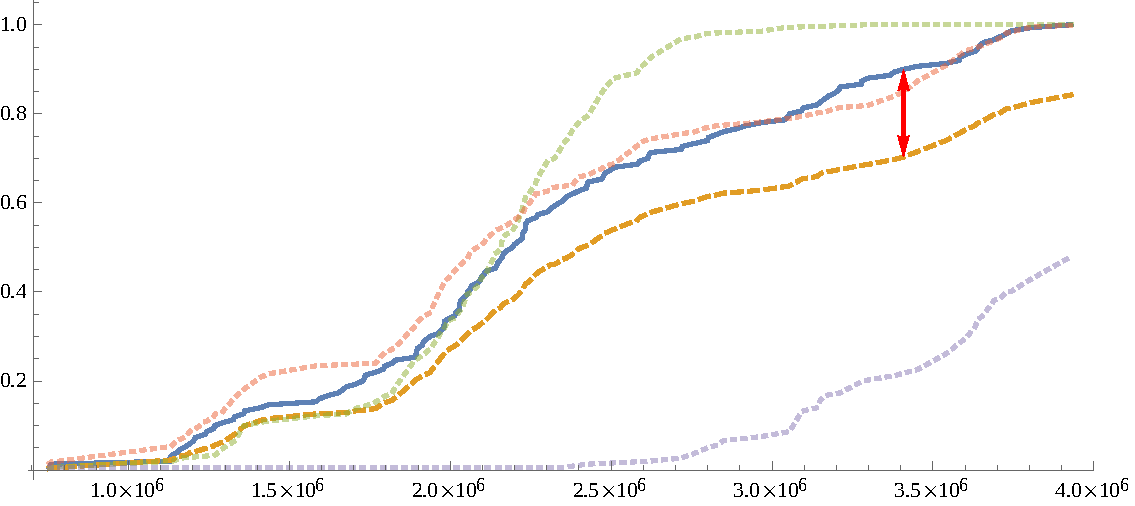
\includegraphics[width=0.4\textwidth,]{Figures/plot-delaunay-example-prediction.pdf}};
    \node[below=of img, node distance=1cm, yshift=1cm] {I/O Throughput};
    \node[left=of img, node distance=0cm, rotate=90, anchor=center,yshift=-0.7cm] {CDF Value};
  \end{tikzpicture}
  \vspace{-0.3cm}
  \caption{In this HPC I/O example, the general methodology for predicting a CDF and evaluating error can be seen. The Delaunay method chose three source distributions (dotted lines) and assigned weights \{.3, .4, .3\} (top to bottom at arrow). The weighted sum of the three known CDFs produces the predicted CDF (dashed line). The KS Statistic (arrow) computed between the true CDF (solid line) and predicted CDF (dashed line) is 0.2 for this example. The KS test null hypothesis is rejected at $p$-value 0.01, however it is not rejected at $p$-value 0.001.
  \vspace{-.1cm}}
  \label{fig:prediction_example}
\end{figure}

%% ===================================================================
\subsection{Measuring Error}

When the range of an approximation is the real numbers, error is reported with summary statistics including: min absolute error, max absolute error, absolute error quartiles, and mean absolute error. In general, all errors are recorded as signed relative error and any figures depicting distributions of errors will present these values.

A hurdle when modeling function-valued outputs such as cumulative distribution functions (CDFs) or probability density functions (PDFs) is that certain properties must be maintained. It is necessary that a PDF $f: \mathbb{R} \rightarrow \mathbb{R}$ have the properties $f(x) \geq 0$ and $\int_{-\infty}^{\infty}f(x)dx = 1$. However, for a CDF $F: \mathbb{R} \rightarrow \mathbb{R}$ the properties are $F(x) \in [0,1]$ and $F(x)$ is absolutely continuous and nondecreasing. This work utilizes the fact that a convex combination of CDFs (or PDFs) results in a valid CDF. Given $G(x) = \sum_{i}w_i F_i(x)$, $\sum_{i} w_i = 1$, $w_i \geq 0$, and each $F_i$ is a valid CDF, $G$ must also be a valid CDF. A demonstration of how this is applied can be seen in Figure \ref{fig:prediction_example}.

%% %% ===================================================================
%% \subsection{Feature Weighting}
%% \label{sec:feature_weighting}

%% It is well-known that an important procedure in any application of predictive methodologies is identifying those features of the data that are most relevant to making accurate predictions \cite{guyon2003introduction}. Selection strategies such as the floating searches studied in \cite{pudil1994floating} or others compared in \cite{ferri1994comparative} can be too expensive for large approximation problems. Rather, this work poses feature selection as a continuous optimization problem. Let $X$ be an $n \times d$ matrix of $n$ known system configurations with $d$ parameters each normalized to be in $[0,1]$. Define an error function that computes the error of a predictive model trained on $X\hbox{ diag }w$, $w \in \mathbb{R}^d$,  by performing ten random splits with 80\% of the rows of $X\hbox{ diag }w$ for training and 20\% for testing. A minimum of this error function could be considered an optimal weighting of the features of $X$. Minimization is performed using a zero order method in the absence of a readily computable gradient.

%% ===================================================================

The performance of approximation techniques that predict probability functions can be analyzed through a variety of summary statistics. This work uses the max absolute error, also known as the Kolmogorov-Smirnov (KS) statistic \cite{lilliefors1967kolmogorov} for its compatibility with the KS test.

The two-sample KS test is a useful nonparametric test for comparing two CDFs while only assuming stationarity, finite mean, and finite variance. The null hypothesis (that two CDFs come from the same underlying distribution) is rejected at level $p \in [0,1]$ when
$$ KS > \sqrt{-\frac{1}{2}\ln\biggl(\frac{p}{2}\biggr)} \sqrt{\frac{1}{n_1} + \frac{1}{n_2}}, $$
with distribution sample sizes $n_1,n_2 \in \mathcal{N}$. For all applications of the KS test presented in this work $n_1 = n_2$. An example of the round-trip prediction methodology from known and predicted distributions to the calculation of error can be seen in Figure \ref{fig:prediction_example}.

\section{Theoretical Error Bound}

This section presents the theoretical results bounding the error of Delaunay interpolation. The error analysis relies on the Delaunay interpolation for two reasons: (1) second order results can be obtained utilizing a Lipschitz constant on the gradient of a function, rather than standard Lipschitz bounds and (2) multiple other interpolants analyzed compute predictions as convex combinations of observed function values, which may allow for straight forward extensions of this error bound.

$ $

\noindent \textbf{\textit{Lemma 1.}} Let $S \subset \mathbb{R}^d$ be open and convex, $f: \mathbb{R}^d \rightarrow \mathbb{R},$ and $\nabla f \in Lip_{(\gamma,\|\cdot\|_2)}(S)$, the set of $\gamma$-Lipschitz continuous functions in the $2$-norm. Then for all $x,y \in S$
%
$$\big|f(y) - f(x) - \langle \nabla f(x), y - x \rangle \big| \leq \frac{\gamma \|y - x\|_2^2}{2}.$$

\noindent \textit{Proof.} Consider the function $g(t) = f \big((1-t) x + t y \big),$ $0 \leq t \leq 1,$ whose derivative $g'(t) = \big\langle \nabla f \big((1-t) x + t y \big), y - x \big\rangle$ is the directional derivative of $f$ in the direction $(y - x).$
%
\begin{align*}
  \big|f(y) - f(x) - \langle \nabla f(x), y - x \rangle \big|
     &= \big|g(1) - g(0) - g'(0) \big| & \\
     &= \bigg| \int_0^1 g'(t) - g'(0)\ dt \bigg| \\
     &\leq \int_0^1 \big|g'(t) - g'(0)\big|\ dt \\
     &= \int_0^1 \bigg| \big \langle \nabla f\big((1-t)x + ty\big) - \nabla f(x), y - x \big \rangle \bigg|\ dt \\
     &\leq \int_0^1 \big \| \nabla f\big((1-t)x + ty\big) - \nabla f(x) \big \|_2\ \| y - x \|_2\ dt \\
     &\leq \int_0^1 \big ( \gamma\ \|y-x\|_2 \big) \ \big( \|y-x\|_2 \big) t\ dt \\
     &= \frac{\gamma \|y - x\|_2^2}{2}.
\end{align*}
%
\qed

\noindent \textbf{\textit{Lemma 2.}} Let $x, y, v_i \in \mathbb{R}^d,$ $c_i \in \mathbb{R},$ and $|\langle y - x, v_i \rangle| \leq c_i$ for $i = 1,$ $\ldots,$ $d.$ If $M = (v_1,$ $\ldots,$ $v_d)$ is nonsingular, then
%
$$\|y - x\|_2^2 \leq \frac{1}{\sigma_d^2} \sum_{i=1}^d c_i^2,$$
%
where $\sigma_d$ is the smallest singular value of $M.$

\noindent \textit{Proof.} Using the facts that $M$ and $M^t$ have the same singular values, and $\|M^tw\|_2 \geq \sigma_d \|w\|_2,$ gives
%
\begin{align*}
     \|y - x\|_2^2 &\leq \frac{\|M^t (y - x)\|_2^2}{\sigma_d^2} \\
                   &=    \frac{1}{\sigma_d^2} \sum_{i=1}^d \langle y - x, v_i \rangle^2 \\
                   &\leq \frac{1}{\sigma_d^2} \sum_{i=1}^d c_i^2.
\end{align*}
%
\qed

\noindent \textbf{\textit{Lemma 3.}} Given $f,$ $\gamma,$ $S$ as in {\it Lemma 1}, let $X = \{x_0,$ $x_1,$ $\ldots,$ $x_d\}$ $\subset S$ be the vertices of a $d$-simplex, and let $\hat f(x) = \langle c, x - x_0 \rangle + f(x_0),$ $c \in \mathbb{R}^d$ be the linear function interpolating $f$ on $X.$ Let $\sigma_d$ be the smallest singular value of the matrix $M = (x_1 - x_0,$ $\ldots,$ $x_d - x_0),$ and $k = \max\limits_{1\ \leq\ j\ \leq\ d} \|x_j - x_0\|_2.$ Then
%
$$\big\|\nabla f(x_0) - c\big\|_2 \leq \sqrt{d} \frac{\gamma k^2}{\sigma_d}.$$

\noindent \textit{Proof.} Consider $f(x) - \hat f(x)$ along the line segment $z(t) = (1-t)x_0 + t x_j,$ $0 \leq t \leq 1.$ By Rolle's Theorem, for some $0 < \hat t < 1,$ $\big\langle \nabla f\big(z(\ \hat t\ )\big) - c, x_j - x_0 \big\rangle = 0.$ Now
%
\begin{align*}
  \big| \big< \nabla f(x_0) - c, x_j - x_0 \big \rangle \big|
        &= \big| \big< \nabla f(x_0) - \nabla f\big(z(\ \hat t\ )\big) + \nabla f\big(z(\ \hat t\ )\big) - c, x_j - x_0 \big \rangle \big| \\
	&= \big| \big\langle \nabla f(x_0) - \nabla f \big(z(\ \hat t\ )\big), x_j - x_0 \big \rangle \big| \\
	&\leq \big \| \nabla f(x_0) - \nabla f\big(z(\ \hat t\ )\big) \big \|_2 \|x_j - x_0\|_2 \\
	&\leq \gamma \|x_0 - z(\ \hat t\ )\|_2\ \|x_j - x_0\|_2 \\
	&\leq \gamma \|x_j - x_0\|_2^2 \leq \gamma k^2, \\
\end{align*}
%
for all $1 \leq j \leq d.$ Using {\it Lemma 2},
%
$$\big \| \nabla f(x_i) - c \big \|_2^2 \leq \frac{d}{\sigma_d^2} \big( \gamma k^2\big)^2 \implies \big \| \nabla f(x_i) - c \big \|_2 \leq \sqrt{d} \frac{\gamma k^2}{\sigma_d}.$$
%
\qed

\noindent \textbf{\textit{Theorem.}} Under the assumptions of {\it Lemma 1} and {\it Lemma 3}, for $z \in S,$
%
$$ \big|f(z) - \hat f(z)\big| \leq \frac{\gamma \|z - x_0\|_2^2}{2} + \sqrt{d} \frac{\gamma k^2}{\sigma_d} \|z - x_0\|_2.$$

\noindent \textit{Proof.} Let $v = \nabla f(x_0) - c,$ where $\|v\|_2 \leq \sqrt{d} \gamma k^2 / \sigma_d$ by {\it Lemma 3}. Now
%
\begin{align*}
  \big|f(z) - \hat f(z)\big|
       &= \big|f(z) - f(x_0) - \langle c, z - x_0 \rangle \big| \\ 
       &= \big|f(z) - f(x_0) - \langle \nabla f(x_0) - v, z - x_0 \rangle \big| \\
       &= \big|f(z) - f(x_0) - \langle \nabla f(x_0) , z - x_0 \rangle + \langle v , z - x_0 \rangle \big| \\
       &\leq \big|f(z) - f(x_0) - \langle \nabla f(x_0) , z - x_0 \rangle \big| + \big| \langle v , z - x_0 \rangle \big| \\
       &\leq \big|f(z) - f(x_0) - \langle \nabla f(x_0) , z - x_0 \rangle \big| + \|v\|_2 \|z - x_0\|_2 \\
       &\leq \big|f(z) - f(x_0) - \langle \nabla f(x_0), z - x_0 \rangle \big| + \textstyle{\frac{\gamma k^2 \sqrt{d}}{\sigma_d}} \|z - x_0\|_2 \\
       &\leq \frac{\gamma \|z - x_0\|_2^2}{2} + \sqrt{d}\frac{\gamma k^2}{\sigma_d} \|z - x_0\|_2,
\end{align*}
%
where the last inequality follows from {\it Lemma 1}.
%
\qed

\section{Planning for Paper}

\begin{itemize}
\item Construct analytic function to test theoretical claims made about Delaunay.
\item Demonstrate the empirical performance of Delaunay, discuss alignment with theory.
\item Demonstrate similar empirical performance is achieved by other interpolants.
\item Argue that interpolation is not as commonly applied, but that it works well in practice.
\item Present the data for predicting real-valued outputs, an empirical study.
  \begin{itemize}
  \item Forest fire data
  \item Parkinsons
  \item https://www.kaggle.com/jsphyg/weather-dataset-rattle-package
  \end{itemize}
\item Present prediction results on each of these data sets for each algorithm.
\item Discuss the results between the regressors and interpolants.
\item Present the data for predicting function-valued outputs, an empirical study.
  \begin{itemize}
  \item VarSys large scale system configuration prediction
  \item \textit{galaxy data from Carnegie Melon?}
  \end{itemize}
\item Present prediction results on each of these data sets for each algorithm.
\item Discuss the results between the regressors and interpolants.
\item Present a summary table showing the performance differences between regerssors and interpolants.
\item Discuss the overall applicability of interpolants and encourage further application. Restate the benefits of interpolants
\item Conclude
\end{itemize}

%% \begin{table}
%%   \centering
%%   \begin{tabular}{c|c|c|c|c|c}
%%     \multicolumn{6}{c}{\textit{I/O Zone Distribution Prediction}}\\
%%     Algorithm & Min & $25^{th}$ & $50^{th}$ & $75^{th}$ & Max\\
%%     \hline
%%     Delaunay & \textbf{2.869e-02} & \textbf{9.143e-02} & \textbf{1.582e-01} & 3.084e-01 & 8.974e-01\\
%%     Voronoi & 3.032e-02 & 1.002e-01 & 1.647e-01 & \textbf{2.743e-01} & \textbf{7.621e-01}\\
%%     BoxMesh & 7.035e-02 & 4.172e-01 & 5.611e-01 & 7.447e-01 & 1.000e+00\\
%%     ShepMod & 3.071e-02 & 9.828e-02 & 1.637e-01 & 3.348e-01 & 1.000e+00\\
%%   \end{tabular}
%%   \caption{}
%%   \label{table:}
%% \end{table}



\section{Data and Analysis}
In order to evaluate the proposed interpolation and approximation techniques, this paper utilizes three data sets of varying dimension and application. In the following subsections the sources and targets of each data set are described, as well as challenges and limitations related to interpolating and approximating these data sets. The distributions of response values being modeled can be seen in Figure \ref{fig_response_hists}. The preprocessing and approximation processes are described in Section \ref{sec_performance_analysis}.

\begin{figure}
  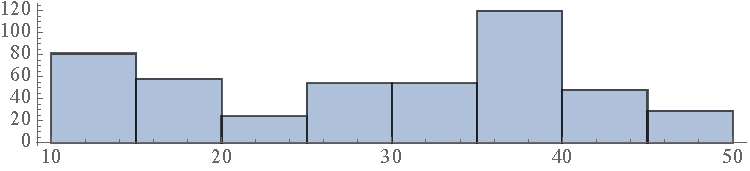
\includegraphics[width=.5\textwidth,height=2cm]{Figures/p-hist.pdf}
  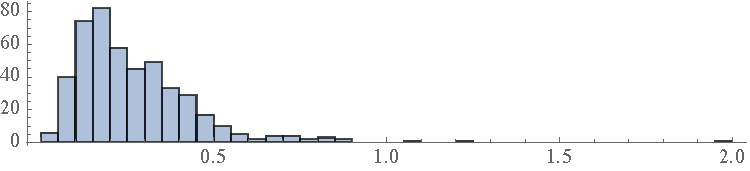
\includegraphics[width=.5\textwidth,height=2cm]{Figures/f-hist.pdf}
  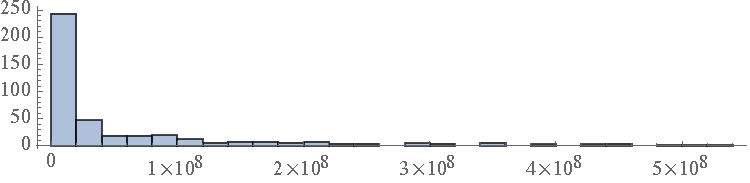
\includegraphics[width=.5\textwidth,height=2cm]{Figures/h-hist.pdf}
  \caption{Histograms of Parkinsons (total UPDRS), forest fire (area), and HPC I/O (mean throughput) response values respectively. Notice that both the forest fire and HPC I/O data sets are heavily skewed.
  \vspace{-.5cm}}
  \label{fig_response_hists}
\end{figure}

\subsection{Data Summary}

\subsubsection{High Performance Computing I/O ($n = 532, d = 4$)}
The first of three data sets is a four-dimensional data set produced by executing the IOzone benchmark from \cite{iozone} on a homogeneous cluster of computers. The system performance data was collected by executing IOzone 40 times for each of a select set of system configurations. A single IOzone execution reports the max I/O file-read throughput seen. The 40 executions for each system configuration are converted to their mean, which is capable of being modeled by each of the multivariate approximation techniques presented in Section \ref{sec_mesh_construction}. The four dimensions being modeled to predict throughput mean are file size, record size, thread count, and CPU frequency.

\begin{figure*}[htb]
  \begin{tikzpicture}
    \node (img)  {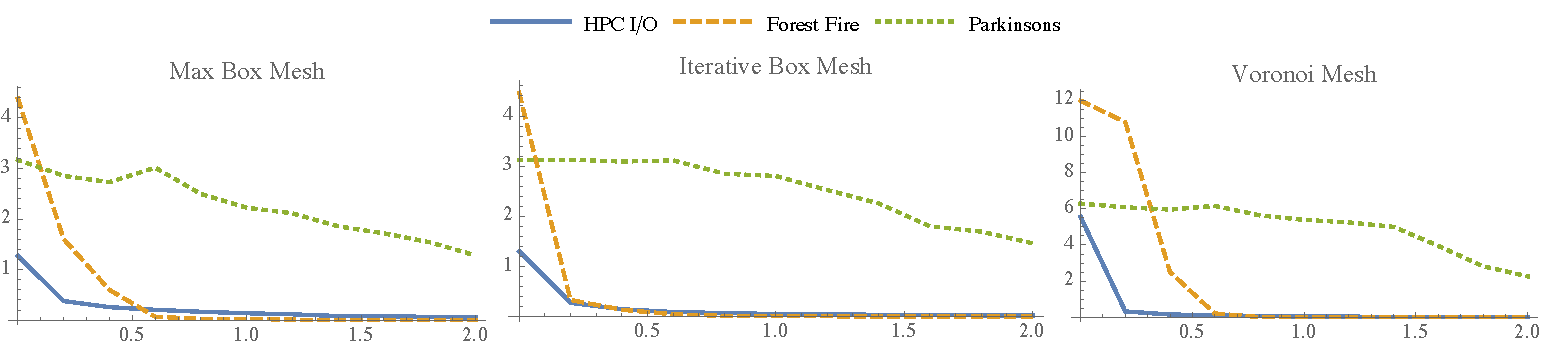
\includegraphics[width=0.95\textwidth,height=4cm]{Figures/eval-times.pdf}};
    \node[below=of img, node distance=0cm, yshift=1cm] {Relative Error Tolerance while Bootstrapping};
    \node[left=of img, node distance=0cm, rotate=90, anchor=center,yshift=-0.7cm] {Fit Time};
  \end{tikzpicture}
  \caption{Time required to generate model fits for each technique with varying relative error tolerance during bootstrapping.
    \vspace{-.3cm}}
  \label{fig_eval_times}
\end{figure*}

\subsubsection{Forest Fire ($n = 517, d = 12$)}
The forest fire data set \cite{cortez2007data} describes the area of Montesinho park burned on specific days and months of the year in terms of the environmental conditions. The twelve dimensions being used to model burn area are the $x$ and $y$ spatial coordinates of burns in the park, month and day of year, the FFMC, DMC, DC, and ISI indices (see source for details), the temperature in Celsius, relative humidity, wind speed, and outdoor rain. The original analysis of this data set demonstrated it to be difficult to model, likely due to the skew in response values.

\subsubsection{Parkinson's Telemonitoring ($n = 468, d = 16$)}
The final data set for evaluation \cite{tsanas2010accurate} is derived from a speech monitoring study with the intent to automatically estimate Parkinson's disease symptom development in Parkinson's patients. The function to be predicted is a time-consuming clinical evaluation measure referred to as the UPDRS score. The total UPDRS score given by a clinical evaluation is estimated through 16 real numbers generated from biomedical voice measures of in-home sound recordings.

\subsection{Performance Analysis}
\label{sec_performance_analysis}

The performance of the approximation techniques varies considerably across the three evaluation data sets. Relative errors for the most na\"{\i}ve approximators such as nearest neighbor can range from zero to $\displaystyle \big(\max_x f(x) - \min_x f(x)\big) / \min_x f(x)$ when modeling a positive function $f(x)$ from data. Each of the approximation techniques presented remain within these bounds and all errors are presented in signed relative form $(\hat f(x) - f(x)) / f(x)$. Before the models are constructed all data values (components $x^{(i)}_r$ of $x^{(i)} \in X$) are shifted and scaled to be in the unit cube $[0,1]^d$, while the response values are taken in their original form. All models are evaluated with $10$ random $80/20$ splits of the data.

\begin{table}
  \centering
  \begin{tabular}{c|c|c|c}
    \hline
    \textbf{Data Set} & \textbf{Technique} & \textbf{Tolerance} & \textbf{Average Error}\\
    \hline
    HPC I/O & MBM & 1.2 & 0.597\\
    Forest Fire & MBM & 1.8 & 3.517\\
    Parkinson's & MBM & 0.6 & 0.114\\
    \hline
    HPC I/O & IBM & 0.4 & 0.419\\
    Forest Fire & IBM & 1.8 & 3.615\\
    Parkinson's & IBM & 1.8 & 0.121\\
    \hline
    HPC I/O & VM & 0.2 & 0.382\\
    Forest Fire & VM & 1.0 & 4.783\\
    Parkinson's & VM & 2.0 & 1.824\\
    \hline
  \end{tabular}
  \caption{The optimal error tolerance bootstrapping parameters for each technique and each data set as well as the average absolute relative errors achieved by that tolerance. Notice that large relative error tolerances occasionally yield even lower evaluation errors, demonstrating the benefits of approximation over interpolation for noisy data sets.
  \vspace{-.5cm}}
  \label{tab_optimal_tolerance}
\end{table}

Each of the approximation techniques presented incorporates bootstrapping based on an allowable error tolerance $t$. An analysis of the effects of bootstrapping error tolerances on validation accuracy can be seen in Figure \ref{fig_all_performance}. The approximation meshes perform best on the forest fire and Parkinson's data sets when the error tolerance used for fitting is large (smoothing rather than interpolating), while near-interpolation generally produces the most accurate models for HPC I/O. Another performance result of note is that the $MBM$ and $IBM$ have very similar basis functions with largely different outputs.

\begin{figure*}
  \begin{tikzpicture}
    \node (img)  {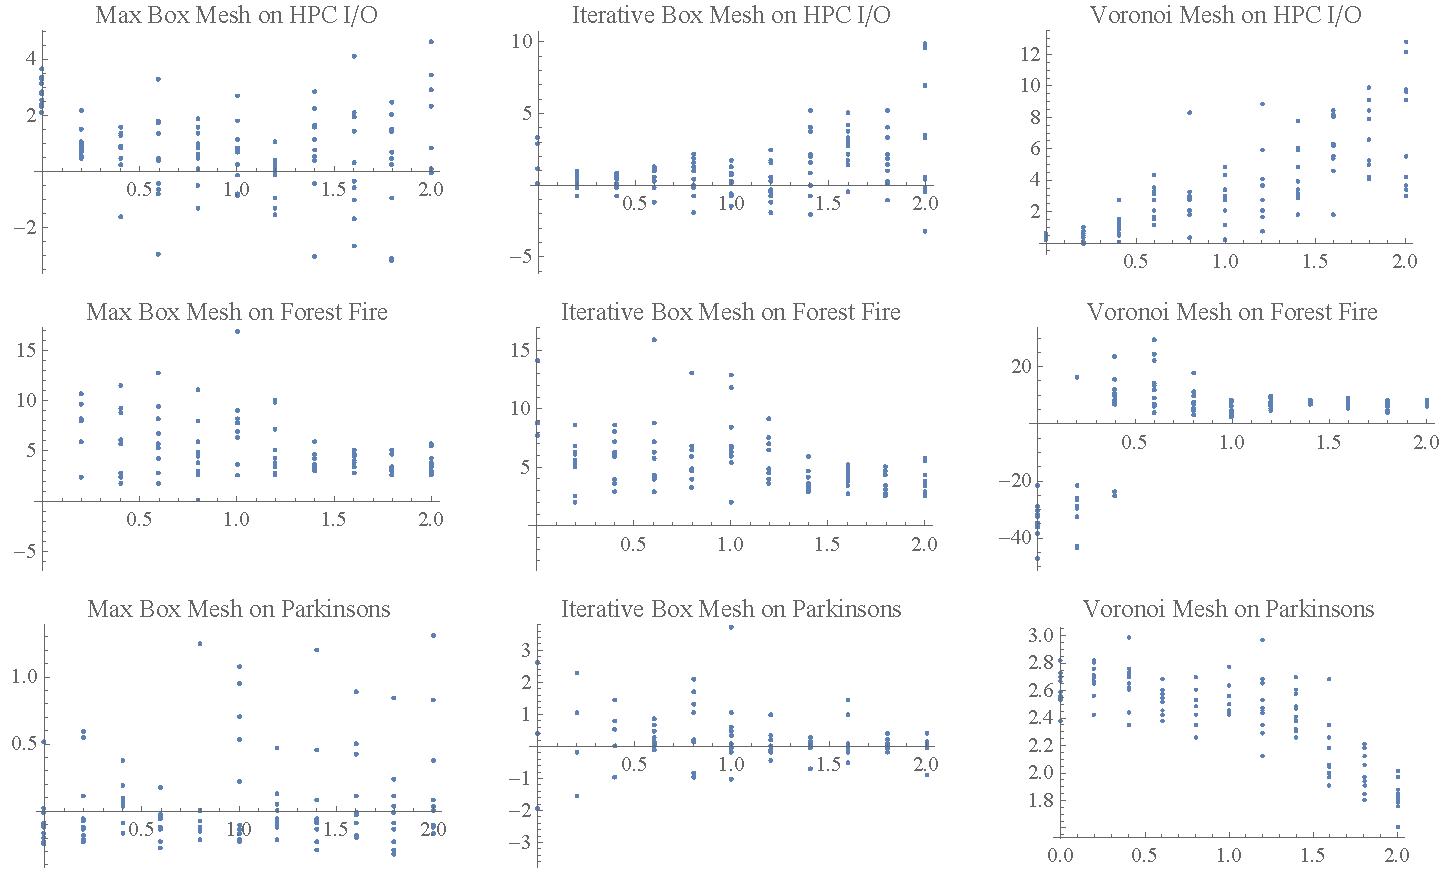
\includegraphics[width=0.95\textwidth,height=9.5cm]{Figures/all-performance.pdf}};
    \node[below=of img, node distance=0cm, yshift=1cm] {Relative Error Tolerance while Bootstrapping};
    \node[left=of img, node distance=0cm, rotate=90, anchor=center,yshift=-0.7cm] {Signed Relative Error};
  \end{tikzpicture}
  \caption{The performance of all three techniques with varied relative error tolerance for the bootstrapping parameter. The columns are for Max Box Mesh, Iterative Box Mesh, and Voronoi Mesh, respectively. The rows are for HPC I/O, Forest Fire, and Parkinson's respectively. Notice the techniques' behavior on the Parkinson's and Forest Fire data sets, performance increases with larger error tolerance.}
  \label{fig_all_performance}
\end{figure*}

\begin{figure*}
  \begin{tikzpicture}
    \node (img)  {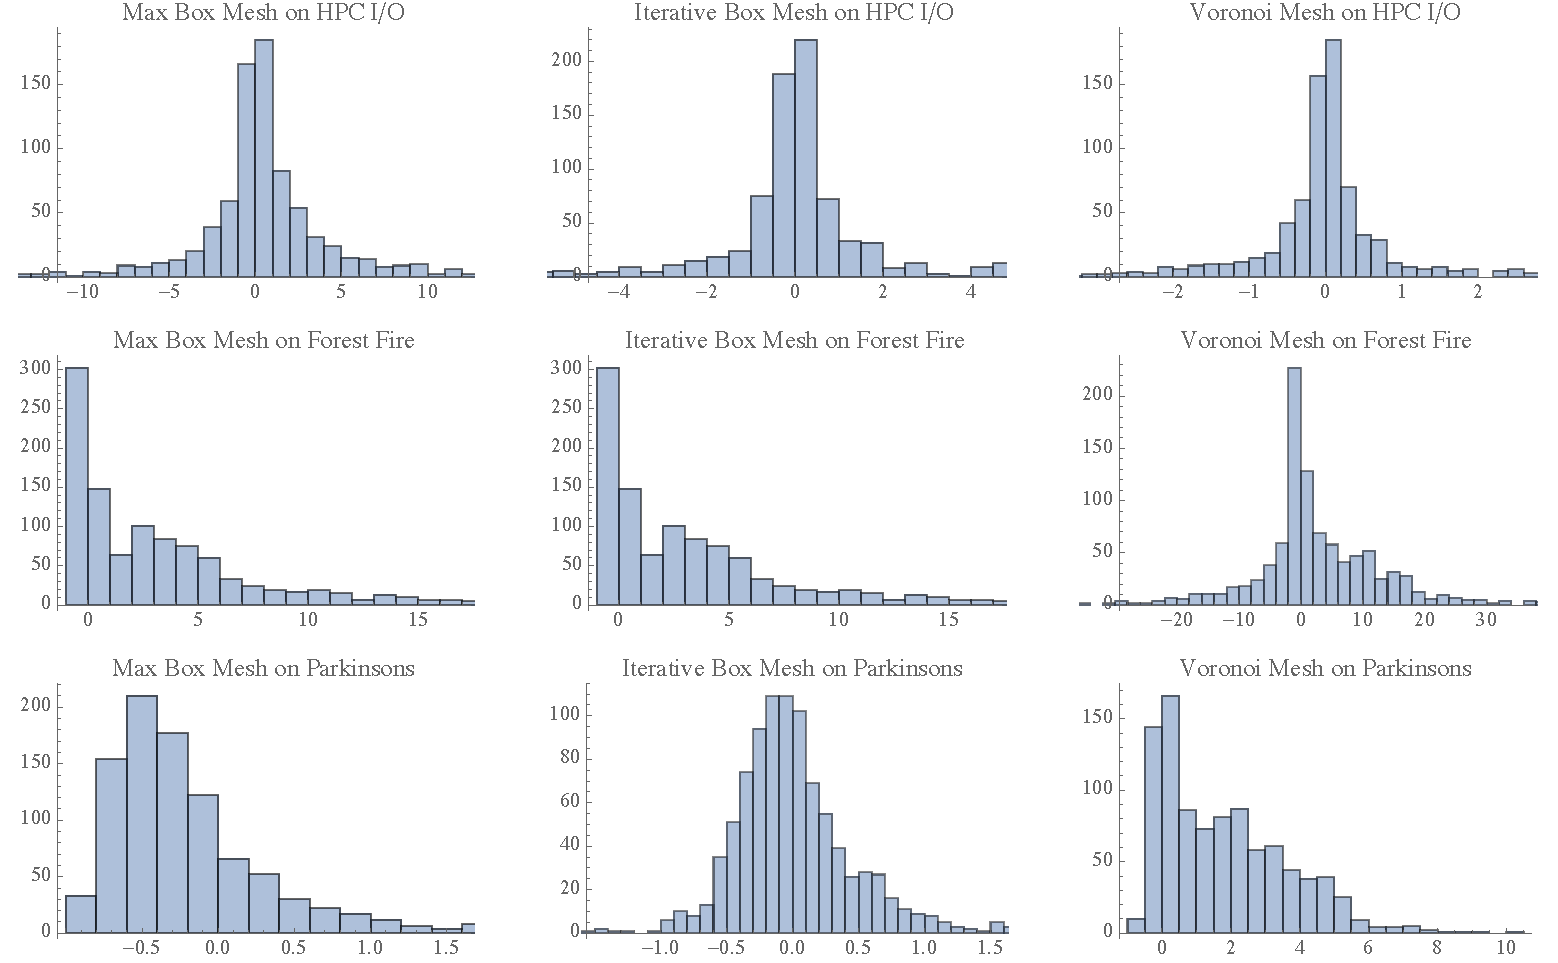
\includegraphics[width=0.95\textwidth,height=9.5cm]{Figures/perf-sample.pdf}};
    \node[below=of img, node distance=0cm, yshift=1cm] {Signed Relative Error in Prediction};
    \node[left=of img, node distance=0cm, rotate=90, anchor=center,yshift=-0.7cm] {Count};
  \end{tikzpicture}
  \caption{A sample of relative errors for all three techniques with optimal selections of error tolerance. The columns are for Max Box Mesh, Iterative Box Mesh, and Voronoi Mesh, respectively. The rows are for HPC I/O, Forest Fire, and Parkinson's respectively.
    \vspace{-.3cm}}
  \label{fig_perf_sample}
\end{figure*}

The selection of bootstrapping error tolerance also effects the computation time required to fit each of the models to data. Figure \ref{fig_eval_times} presents the time required to construct approximations for each model and each data set with varying $t$. The rapid reduction in computation time required for the forest fire and HPC I/O data sets suggests that large reductions in error can be achieved with relatively few basis functions. The Parkinson's data set however presents a more noisy response, with increasing number of basis functions reducing error much less quickly.

The distributions of errors experienced by each approximation technique when the optimal bootstrapping relative error tolerance is selected can be seen in Figure \ref{fig_perf_sample}. HPC I/O exhibits the most normal approximation errors, which suggests that the models are converging on the random noise of the response for the data set. The worst relative approximation errors are produced by the Voronoi mesh on the forest fire data set. The small magnitude true response values contribute to the larger relative errors. Regardless, the $VM$ errors are unacceptably large.

\section{Discussion}

The bootstrapping procedure presented for each approximation technique still has much room for improvement. Initial analysis suggests that the appropriate relative error tolerance needs to be discovered empirically for each application of a modeling technique. Further analytic studies could arrive at methods for determining optimal error tolerances at runtime, however increases in runtime complexity may not be afforded in many applications. 

The box-shaped basis functions and the construction algorithms used for the $MBM$ and $IBM$ could become a source of error when $d$ (the dimension of the data $X$) is comparable to $n$ (the number of known points). The blending regions in which multiple basis functions overlap are always axis aligned and in applications such as image analysis, any single dimension may be unsuitable for approximating the true underlying function. The Voronoi mesh attempts to address this problem by utilizing boundaries between points in multiple dimensions simultaneously. However, it is empirically unclear whether the true benefits of the $VM$ are seen in applications where $d \ll n$.

Each of the case studies presented have fewer than $1000$ points. The complexities of the presented approximation techniques are suitable for large dimension, but the increased complexity associated with brute-force bootstrapping currently prohibits their use on larger data sets. The Voronoi mesh in particular has a large complexity with respect to $n$ which could be significantly improved via more greedy bootstrapping. While each technique requires less than ten seconds on average to produce a fit in the presented case studies, the fit time required quickly grows into minutes around $1000$ points. While these initial results appear somewhat limiting, they demonstrate the viability of each mesh and leave room for further theoretical exploration of techniques to reduce the runtime complexity while maintaining the approximation power and flexibility.

\section{Conclusion}

The Max Box Mesh, Iterative Box Mesh, and Voronoi Mesh each provide novel strategies for effectively approximating multivariate phenomonon. The underlying constructions are theoretically straightforward, yet powerful and flexible. The computational complexities of each make them particularly suitable for applications in many dimensions, while the bootstrapping error tolerance parameter allows a balance between smoothing and interpolation to be explored empirically with each application.

\subsection{Future Work}

A thorough comparison with constituent multivariate approximation techniques including but not limited to, linear Shepard interpolation, multivariate adaptive regression splines, multilayer perceptron regression, and Delaunay triangulation constitutes future work. A more detailed study of alternative bootstrapping techniques may also provide valuable insight.




%%%%%%%%%%%%%%%%%%%%%%%%%%%%%%%%%%%%%%%%%%%%%%%%%%%%%%%%%%%%%%%%%%%%%%%%%%%%%%%%


%% ===================================================================
\section{DATA}
\label{sec:data}

\begin{table}
  \centering
  \begin{tabular}{c|c}
    \hline
    \textbf{System Parameter} & \textbf{Values}\\
    \hline
    File Size (KB) & 4, 16, 64, 256, 1024, 4096, 8192, 16384\\
    \hline
    Record Size (KB) & \multilinecell{4, 8, 16, 32, 64, 128, 256, 512,\\ 1024, 2048, 4096, 8192, 16384}\\
    \hline
    Thread Count & 1, 8, 16, 24, 32, 40, 48, 56, 64\\
    \hline
    Frequency (GHz) & 1.2, 1.6, 2, 2.3, 2.8, 3.2, 3.5\\
    \hline
    Test Type & \multilinecell{Readers, Rereaders, Random Readers, \\ Initial Writers, Rewriters, Random Writers}\\
    \hline
  \end{tabular}
  \caption{A description of system parameters considered for IOzone. Record size must be $\leq$ file size during execution.
    \vspace{-.5cm}}
  \label{tab:data_description}
\end{table}

\begin{figure}
  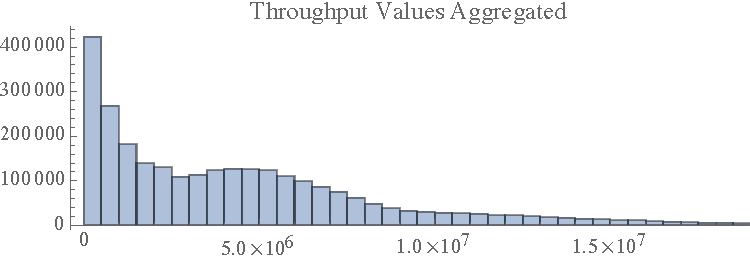
\includegraphics[width=.5\textwidth]{Figures/plot-histogram-throughput.pdf}
  \caption{Histogram of the raw throughput values recorded during all IOzone tests across all system configurations. The distribution is skewed right, with few tests having significantly higher throughput than most others.
  \vspace{-.5cm}}
  \label{fig:throughput_histogram}
\end{figure}

This paper presents a variability modeling case study with a five-dimensional dataset produced by executing the IOzone benchmark \cite{iozone} on a homogeneous cluster of computers. Each node contains two Intel Xeon E5-2637 CPUs offering a total of 16 CPU cores with 16GB of DRAM. While the CPU frequency varies depending on the test configuration, the I/O from IOzone is performed by an ext4 filesystem sitting above an Intel SSDSC2BA20 SSD drive. At the time of data collection, Linux kernel Version 4.13.0 was used. The system performance data was collected over two weeks by executing IOzone 150 times for each of a select set of approximately 18K system configurations, for a total of approximately 2.7M executions of IOzone. A single IOzone execution reports the max I/O throughput in kilobytes per second seen for the selected test type. The summary of the data components in $x^{(i)}$ for the experiments for this paper can be seen in Table \ref{tab:data_description}. Distributions of raw throughput values being modeled can be seen in Figure \ref{fig:throughput_histogram}.

Some mild preprocessing was necessary to prepare the data for modeling and analysis. All features were shifted by their minimum value and scaled by their range, mapping each feature independently into $[0,1]$. This normalization ensures each feature is treated equally by the interpolation techniques and should be performed on all data before building models and making predictions regardless of application. All 150 repeated trials for a system configuration were grouped with that configuration. The only nonordinal feature in this data is the test type. All test types were treated as different applications and were separated for modeling and analysis, i.e., predictions for the ``readers'' test type were made using only known configurations for the ``readers'' test type.

%% ===================================================================

\begin{figure}
  \begin{tikzpicture}
    \node (img)  {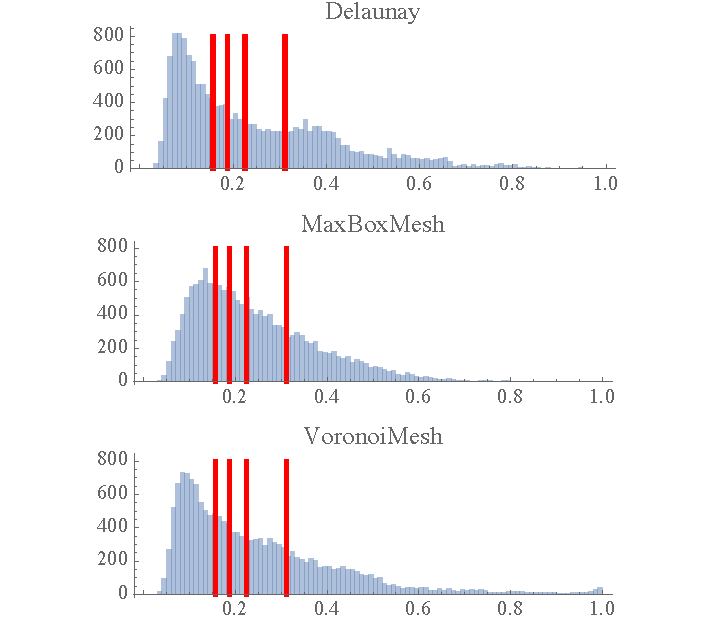
\includegraphics[width=0.5\textwidth,trim={1.5cm 0 0 0}]{Figures/plot-histogram-80_20-KS.pdf}};
    \node[below=of img, node distance=1cm, yshift=1cm] {KS Statistic for Predicted vs. Actual};
    \node[left=of img, node distance=0cm, rotate=90, anchor=center,yshift=-0.7cm] {Count of Predictions with Given KS Statistic};
  \end{tikzpicture}
  \caption{Histograms of the prediction error for each modeling algorithm from ten random splits when trained with 80\% of the data aggregated over all different test types. The distributions show the KS statistics for the predicted throughput distribution versus the actual throughput distribution. The four vertical red lines represent commonly used $p$-values \{0.05, 0.01, 0.001, 1.0e-6\} respectively. All predictions to the right of a red line represent CDF predictions that are significantly different (by respective $p$-value) from the actual distribution according to the KS test.
  \vspace{-.1cm}}
  \label{fig:ks_histogram_80_20}
\end{figure}

\section{RESULTS}
\label{sec:results}

All three interpolation techniques are used to predict the distribution of I/O throughput values at previously unseen system configurations. In order to improve robustness of the error analysis, ten random selections of 80\% of the IOzone data are used to train each model and the remaining 20\% provide approximation error for each model. The recorded errors are grouped by unique system configuration and then averaged within each group. The samples are identical for each interpolation technique, ensuring consistency in the training and testing sets.

The aggregation of errors across all IOzone tests given 80\% of the data as training can be seen in Figure \ref{fig:ks_histogram_80_20}. Agglomerate errors for each technique resemble a Gamma distribution. The percentages of significant prediction errors with varying $p$-values are on display in Table \ref{tab:p_value_failure_rate}. The primary $p$-value used for analyses in this work is 0.001, chosen because close to 2K predictions are made for each test type. Also, applications executed in cloud and HPC systems that could benefit from statistical modeling will be executed at least thousands of times. In line with this knowledge, it is important to ensure that only a small fraction of interpretable results could occur solely under the influence of random chance. When considering the $p=0.001$ results for each technique, a little under half of the predicted CDFs are significantly different from the measured (and presumed) correct CDFs. A rejection rate of 45\% would seem a poor result, however in this situation the complexity of the problem warrants a slightly different interpretation. These predictions are a very \textit{precise} characterization of performance variability, in fact the cumulative distribution function of a random variable is the strongest possible characterization of variability that can be predicted. Globally, only a little under half of the predictions fail to capture \textit{all} of the characteristics of performance variability at new system configurations. It is also demonstrated later in this Section that this result can likely be improved.

\begin{table}
  \centering
  \begin{tabular}{c|c|c}
    \hline
    \textbf{Algorithm} & \textbf{$P$-Value} & \textbf{\% N.H. Rejections} \\
    \hline
    \multilinecell{Delaunay\\Max Box Mesh\\Voronoi Mesh} & .05 & \multilinecell{58.4\\69.3\\61.9}\\
    \hline
    \multilinecell{Delaunay\\Max Box Mesh\\Voronoi Mesh} & .01 & \multilinecell{51.1\\58.4\\53.4}\\
    \hline
    \multilinecell{Delaunay\\Max Box Mesh\\Voronoi Mesh} & .001 & \multilinecell{44.1\\46.9\\45.1}\\
    \hline
    \multilinecell{Delaunay\\Max Box Mesh\\Voronoi Mesh} & 1.0e-6 & \multilinecell{31.4\\26.6\\28.7}\\
    \hline
  \end{tabular}
  \caption{Percent of null hypothesis rejections rate by the KS-test when provided different selections of $p$-values. These accompany the percent of null hypothesis rejection results from Figure \ref{fig:ks_histogram_80_20}. 
    \vspace{-.5cm}}
  \label{tab:p_value_failure_rate}
\end{table}


While interpreting null hypothesis rejection rates for these interpolation techniques, it is important to consider how the rejection rate reduces with increasing amounts of training data. Figure \ref{fig:ks_failure_by_training} displays the change in $p=0.001$ null hypothesis rejection rate with increasing density of training data up to the maximum density allowed by this set. Delaunay interpolation provides the best results with the least training data by about 5\%, but these low density rejection rates are unacceptably high (90\%). Figure \ref{fig:ks_failure_by_training} clearly shows that this data set and/or the system variables used in the models of performance variability is inadequate to capture the full variability map from system parameters to performance CDF. Which or both obtains is not clear. A few well chosen data points can significantly improve the interpolants, and thus a careful study of the rejection instances is warranted, besides enlarging the set of system variables being modeled.

It may be misleading to consider the global performance of each prediction technique across all test types, as some test types are more difficult than others to predict and have more apparent latent variables. In Figure \ref{fig:ks_failure_by_training_and_test}, the relative difficulty of each IOzone test type can be compared. The I/O test types analyzing reads are typically approximated with lower error than those test types analyzing writes. Regardless of test type, in the aggregate results the KS statistics hover consistently around 0.15, demonstrating an impressively low KS statistic for predictions. In order to address the opacity of aggregate analysis, another case study and an application of the methodology from Section \ref{sec:feature_weighting} is presented in Table \ref{tab:optimized_p_value_failure_rate}.

\begin{figure}
  \begin{tikzpicture}
    \node (img)  {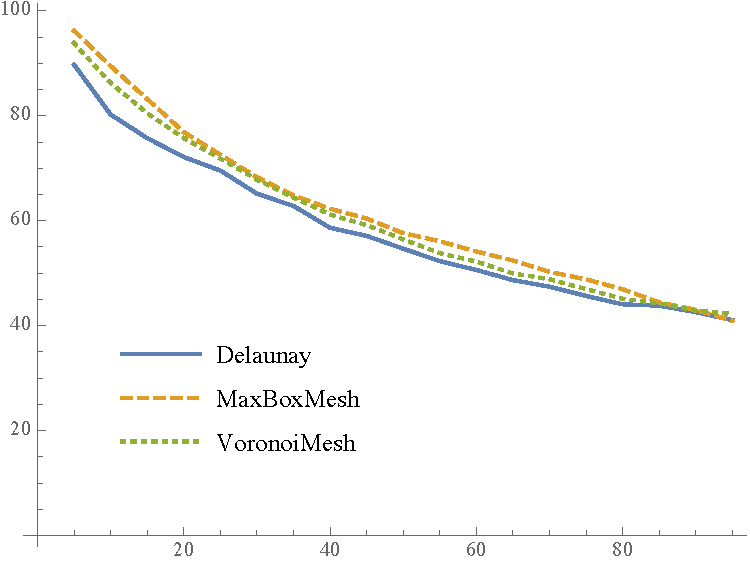
\includegraphics[width=0.4\textwidth,]{Figures/plot-KS-Failure-by-Training.pdf}};
    \node[below=of img, node distance=1cm, yshift=1cm] {Percentage of Training Data};
    \node[left=of img, node distance=0cm, rotate=90, anchor=center,yshift=-0.7cm] {\% Null Hypothesis Rejections};
  \end{tikzpicture}
  \caption{The performance of each algorithm on the KS test ($p=0.001$) with increasing amounts of training data averaged over all IOzone test types and ten random splits of the data. The training percentages range from 5\% to 95\% in increments of 5\%. Delaunay is the best performer until 95\% of data is used for training, at which Max Box mesh becomes the best performer by a fraction of a percent.
  \vspace{-.1cm}}
  \label{fig:ks_failure_by_training}
\end{figure}

The results presented in Table \ref{tab:optimized_p_value_failure_rate} are achieved by permitting each approximation technique 300 iterations of simulated annealing. In each iteration, the impact of potential weights on the average KS statistic were considered. All weights were kept in the range [0,2], and were applied to the normalized features for frequency, file size, record size, and number of threads. All three approximation techniques had similar optimal weights achieved by simulated annealing of approximately $(.001, 2, 1.7, 1.5)$ for frequency, file size, record size, and number of threads, respectively. Recall that each interpolation technique uses small distances to denote large influences on predictions, meaning that frequency was the most important feature when predicting variability for the ``readers'' test type, followed not-so-closely by number of threads, then record size.

The ``readers'' test type results demonstrate that the underlying prediction techniques work and are capable of seeing rejection rates below 5\% when tuned for a given application. It is important to emphasize that the roughly 95\% of predictions for which the null hypothesis was not rejected are predicting the \textit{precise} distribution of I/O throughput that will be witnessed at a previously unseen system configuration. To the authors' knowledge, there is no existing methodology that is generically applicable to any system performance measure, agnostic of system architecture, and capable of making such powerful predictions.

\begin{table}
  \centering
  \begin{tabular}{c|c|c|c}
    \hline
    \textbf{Algorithm} & \textbf{$P$-Value} & \multilinecell{\textbf{Unweighted}\\\textbf{\% N.H. Rejection}} & \multilinecell{\textbf{Weighted}\\\textbf{\% N.H. Rejection}}\\
    \hline
    \multilinecell{Delaunay\\Max Box Mesh\\Voronoi Mesh} & .05 & \multilinecell{24.9\\21.3\\18.7} & \multilinecell{30.2\\21.2\\11.3}\\
    \hline
    \multilinecell{Delaunay\\Max Box Mesh\\Voronoi Mesh} & .01 & \multilinecell{21.6\\16.4\\14.9} & \multilinecell{27.4\\16.4\\7.0}\\
    \hline
    \multilinecell{Delaunay\\Max Box Mesh\\Voronoi Mesh} & .001 & \multilinecell{19.7\\13.1\\12.3} & \multilinecell{25.4\\13.1\\4.6}\\
    \hline
    \multilinecell{Delaunay\\Max Box Mesh\\Voronoi Mesh} & 1.0e-6 & \multilinecell{17.9\\11.3\\8.5} & \multilinecell{23.4\\11.3\\2.3}\\
    \hline
  \end{tabular}
  \caption{The null hypothesis rejection rates for various $p$-values with the KS-test. These results are strictly for the ``readers'' IOzone test type and show unweighted results as well as the results with weights tuned for minimum error (KS statistic) by 300 iterations of simulated annealing. Notice that the weights identified for the Delaunay model cause data dependent tuning, reducing performance. MaxBoxMesh performance is improved by a negligible amount. VoronoiMesh performance is notably improved.
    \vspace{-.5cm}}
  \label{tab:optimized_p_value_failure_rate}
\end{table}

%% \begin{itemize}
%% \item Case studies of good and bad predictions of distributions made, present 3 (best, median, worst)
%% \item Table / Figure showing error for each of the tests (hardest test to predict)
%% \item Presentation of the top most difficult configurations to predict for each test (and the bad performance at those points)
%% %% \item Comparison to predictions made using the "test" numerical column
%% \end{itemize}

\section{DISCUSSION}
\label{sec:discussion}

The results of the IOzone case study indicate that predicting the CDF of I/O throughput at previously unseen system configurations is a challenging problem. The KS statistic captures the worst part of any prediction and hence provides a conservatively large estimate of approximation error. The average absolute errors in the predicted CDFs are always lower than the KS statistics. However, the KS statistic was chosen because of the important statistical theory surrounding it as an error measure. Considering this circumstance, a nonnegligible volume of predictions provide impressively low levels of error. Powerful predictive tools such as those presented in this work allow for more in-depth analysis of system performance variability. For example, system configurations that are most difficult to predict in these tests are likely ``outlier'' configurations that do not resemble those configurations that share many similar parameters. Analysis of these configurations may provide valuable insight into effective application specific operation of computer systems.

As mentioned in Section \ref{sec:introduction}, no prior work has attempted to model an arbitrary performance measure for a system to such a high degree of precision. All previous statistical modeling attempts capture a few ($<3$) ordinal performance measures. Generating models that have such high degrees of accuracy allows system engineers to identify previously unused configurations that present desired characteristics. Service level agreements (SLAs) in cloud computing environments are cause for capital competition that is affected heavily by system performance \cite{patel2009service}. Users prefer SLAs that allow the most computing power per monetary unit, incentivizing service providers to guarantee the greatest possible performance. Overscheduling and irregular usage patterns force cloud service providers to occasionally overload machines, in which case precise models of system performance can be used to statistically minimize the probability of SLA violation. Similar targeted performance tuning techniques can be applied to HPC system configuration to maximize application throughput or minimize system power consumption.

A final application domain affected by this methodology is computer security. Collocated users on cloud systems have received attention recently \cite{ali2015security}. If a malicious collocated user is capable of achieving specific insight into the configuration of the system, or the activity of other collocated users by executing performance evaluation programs (i.e., IOzone), a new attack vector may present itself. Malicious users could be capable of identifying common performance distributions of vulnerable system configurations and vulnerable active user jobs. This knowledge may allow targeted exploits to be executed. Light inspection of raw IOzone I/O throughputs provides substantial evidence that distinct performance distributions coincide closely with specific system configuration parameters. Conversely, a service provider may defend against such attacks by deliberately obfuscating the performance of the machine. Models such as those presented in this paper could identify optimal staggering and time-delay whose introduction into the system would prevent malicious users from identifying system configurations and active jobs.


\begin{figure}
  \begin{tikzpicture}
    \node (img)  {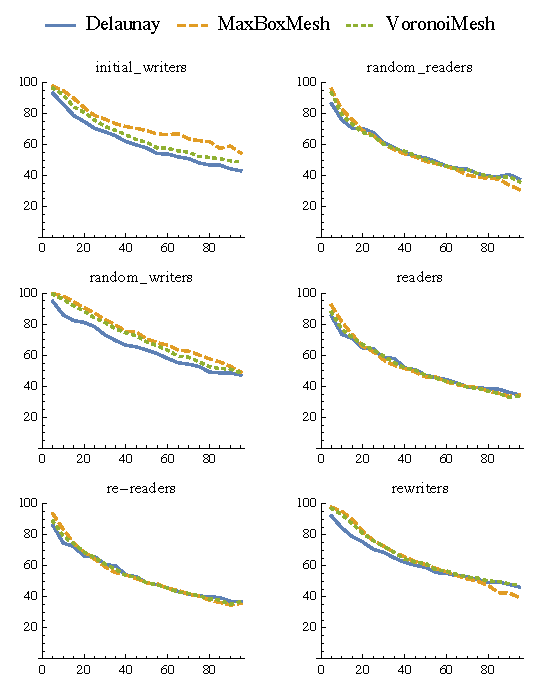
\includegraphics[width=0.4\textwidth,]{Figures/plot-KS-failure-by-training-and-test.pdf}};
    \node[below=of img, node distance=1cm, yshift=1cm] {Percentage of Training Data};
    \node[left=of img, node distance=0cm, rotate=90, anchor=center,yshift=-0.7cm] {\% Null Hypothesis Rejections};
  \end{tikzpicture}
  \caption{The percentage of null hypothesis rejections for predictions made by each algorithm on the KS test ($p=0.001$) over different IOzone test types with increasing amounts of training data. Each percentage of null hypothesis rejections is an average over ten random splits of the data. The training percentages range from 5\% to 95\% in increments of 5\%. The read test types tend to allow lower rejection rates than the write test types.
  \vspace{-.1cm}}
  \label{fig:ks_failure_by_training_and_test}
\end{figure}


Results presented in Table \ref{tab:optimized_p_value_failure_rate} are particularly interesting, demonstrating that Delaunay appears most vulnerable to data dependent tuning, Max Box mesh is largely insensitive to such tuning, and Voronoi mesh benefits (for this data set) from the tuning.

There are many avenues for extending this modeling methodology. One extension is to add categorical variables to the models. Presently the rejection rate of distribution predictions can only be reduced with large volumes of performance data, however the judicious choice (via experimental design, e.g.) of new data points may be able to effectively reduce the amount of training data required. Finally, more case studies need to be done to test the robustness of the present modeling techniques to changes in domain and performance measure.

\section{CONCLUSION}
\label{sec:conclusion}

The methodology presented is capable of providing new insights, extending existing analyses, and improving the management of computational performance variability. Delaunay, Max Box mesh, and Voronoi mesh interpolation are viable techniques for constructing approximations of performance cumulative distribution functions. A case study on I/O throughput demonstrated that the models are capable of effectively predicting CDFs for most unseen system configurations for any of the available I/O test types. The present methodology represents a notable increase in the ability to statistically model arbitrary system performance measures involving the interaction of many ordinal system parameters.
%% \begin{itemize}
%% \item Modeling the distributions of system performance is valuable.
%% \item This work presents a steep increase in the power of predictions made by statistical modeling techniques.
%% \end{itemize}

%\begin{acknowledgements}
%If you'd like to thank anyone, place your comments here
%and remove the percent signs.
%\end{acknowledgements}

%%====================================================================
%%====================================================================

\bibliographystyle{spmpsci}      % mathematics and physical sciences
\bibliography{paper}

\end{document}
